\section{Introduction}

\mode<presentation>{
\begin{frame}
	\frametitle{Introduction}
	\begin{itemize}
		\item<1-> Transaction Level Modeling
		\item<1-> Principles
		\item<1-> TLM1 and TLM2
		\item<1-> Coding Styles
	\end{itemize}
\end{frame}

\begin{frame}
	\frametitle{Introduction: Transaction Level Modeling}
	Objectives:
	\begin{itemize}
		\item<1-> Provide an early platform for software development.
		\item<1-> Aiding software/hardware integration.
		\item<1-> Enabling software performance analysis.
		\item<1-> System Level Design architecture analysis.
		\item<1-> Functional hardware verification.
	\end{itemize}
	The TLM programming model does not try replace the classical SystemC programming style, it tries to enhance it for the previous objectives.
	For cycle level models stick to the classical programming style.
\end{frame}
}

\mode<article>{
In the previous chapter we have seen how to create simulators using SystemC.
While those simulators are very precise, they are pretty slow and difficult to create\footnote{Not that difficult if the different modules are available off the shelf and the only thing you have to do is to assemble them, but difficult otherwise.}.
Additionally, it is difficult to create abstract models using the proposed constructions and syntax (but not impossible).
To solve those issues \emph{Transaction Level Modeling} (aka TLM) has been proposed.
TLM tries to tackle the following problems:
\begin{itemize}
\item Provide an early platform for software development.
\item Aiding software/hardware integration.
\item Enabling software performance analysis.
\item System Level Design architecture analysis.
\item Functional hardware verification.
\end{itemize}
You may think that TLM allows you to build cycle level models, and it is\ldots true.
However, it is not recommended to build cycle level models using TLM for several reasons:
\begin{itemize}
\item You will be reinventing the wheel. 
	SystemC already provides you with support to build cycle level models, so use it. 
	Your cycle level models will be more readable.
\item The SystemC primitives for cycle level modeling can allow the underlying engine to enhance the final simulator.
	If you use TLM to build your cycle level modeling you will be hiding information to the underlying engine, thus limiting the optimization opportunities available to the engine.\footnote{The SystemC reference implementation provided by the Accellera group does not perform any optimization on the simulator, however some commercial and free products/projects do so.
	Maybe the reference implementation will provide them one day.}
\end{itemize}

In this chapter we will study the TLM proposed by the Accellera, and more specifically the latest proposed version: Accellera TLM 2.0.
In this section we will explain a little bit of history about the evolution of the TLM proposals by the Accellera group, and introduce the different coding styles proposed by TLM 2.0.
The following sections will explain the core of TLM 2.0 and how you can use the different coding styles to build your simulators.
}

\subsection{Principles}

\mode<presentation>{
\begin{frame}
	\frametitle{Introduction: Principles}
	\begin{center}
		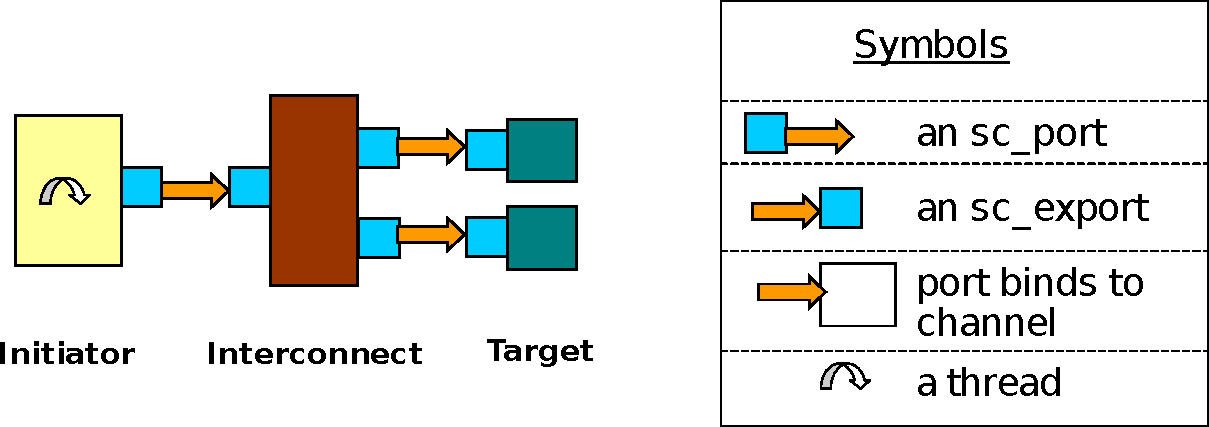
\includegraphics[width=1\textwidth]{tlm/figures/principles.pdf}
	\end{center}
	\begin{itemize}
		\item Modular and hierarchical description (like cycle level)
		\item Communication through \texttt{sc\_port} and \texttt{sc\_export} templated with interfaces
		\item Time locally controlled by modules
		\begin{itemize}
			\item use \texttt{wait(\ldots)} to synchronize with simulation time
		\end{itemize}
	\end{itemize}
\end{frame}
}

\mode<article>{
Like for the cycle level models, TLM allows a hierarchical description of the system where the different components of the system are described in the form of modules.

\begin{figure}[!h]
	\begin{center}
		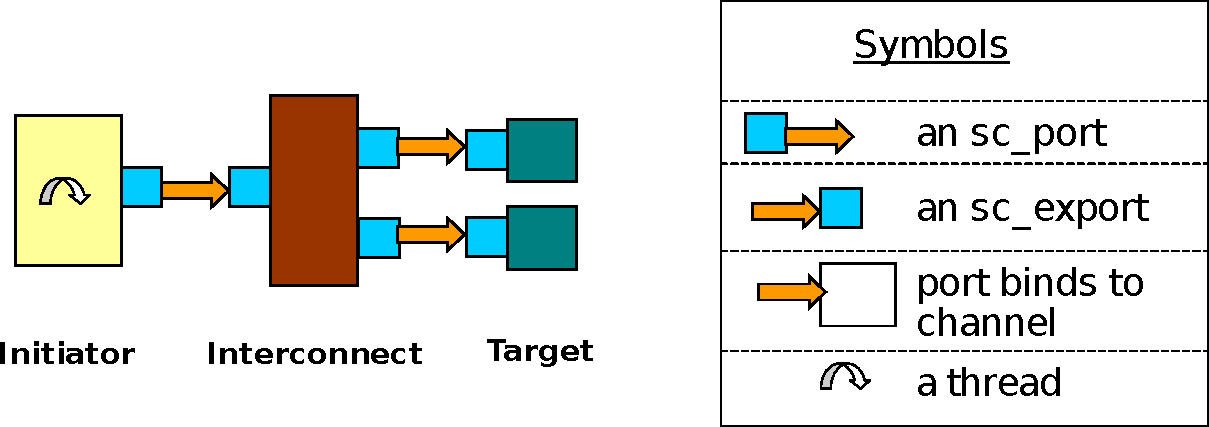
\includegraphics[width=0.8\textwidth]{tlm/figures/principles.pdf}
	\end{center}
	\caption{Example of a TLM system.}
	\label{fig:tlm_principles}
\end{figure}

The modules contain ports through which they communicate.
However the communication is not done through signals, but through direct method calls.
The method calls are defined in interfaces that are associated to the ports.
Initiator modules use the \texttt{sc\_port<>} port types which are templated with the interface they provide.
Likewise, target modules use the \texttt{sc\_export<>} port types which are templated with the interface, interface that the target module must provide an implementation for.
Figure~\ref{fig:tlm_principles} shows an schematic description of those components.

Another particularity of TLM models is that they do not use \texttt{SC\_METHOD} processes, but only \texttt{SC\_THREAD}.
Additionally, modules do not use clock ports to control their time.
Modules keep their local time and use the \texttt{wait(\ldots)} primitive to synchronize themselves with the SystemC global clock, and thus with the rest of the system.
}

\subsection{SystemC 2.0, TLM 1.0 and TLM 2.0}

\mode<presentation>{
\begin{frame}
	\frametitle{Introduction: TLM1 and TLM2}
	\begin{itemize}
		\item<1-> SystemC 1.0 was only adapted to model cycle level simulators
		\item<2-> SystemC 2.0 became an IEEE standard, and introduced new primitives:
		\begin{itemize}
			\item<2-> channels
			\item<2-> events
		\end{itemize}
		TLM models became feasible
		\item<3-> TLM 1.0 provided an untimed framework but message format and timing was missing
		\item<4-> TLM 2.0 improved TLM 1.0 providing:
		\begin{itemize}
			\item<4-> interfaces and methodology for untimed and timed model
			\item<5-> better interoperability with a standard type of message: \emph{\textbf{the generic payload}}
		\end{itemize}
	\end{itemize}	
\end{frame}
}

\mode<article>{
With the release of SystemC 2.0 the Accellera group created new primitives (like channels and events) that offered new programming paradigms to the users.
One of them was Transaction Level Modeling.
However with there were no clear methodology to use those new primitives, which involved compatibility problems when trying to mix TLM models created by different users.
For that purpose the Accellera group created a new working group to define clear interfaces and methodology to create TLM models.
The results of such effort was the first version of TLM in 2005: TLM 1.0.

TLM 1.0 was a clear advance to solve the interoperability issues of existing TLM models.
However, it rapidly started to show its limitations.
The proposed interfaces and methodology were mainly focused on untimed models, it was ill adapted to the development of timed models.
Timed TLM models were possible, however the methodology for creating such models was not defined, which again caused interoperability problems.
For such reason the TLM Accellera working group continued their discussions and released TLM 2.0 in June 2008.
TLM 2.0.2 has since been integrated in IEEE 1666-2011 standard.

With TLM 2.0 the Accellera provides clear interfaces and methodology to create untimed and timed models, and combine them.
Additionally, to increase the interoperability a standard type of message has been defined: \emph{the generic payload}.
We will study the interfaces and methodology provided by TLM 2.0 in the following sections, however, before doing so, we should introduce what are called \emph{coding styles}.
}

\subsection{Coding Styles}

\mode<presentation>{
\begin{frame}
	\frametitle{Introduction: Coding Styles}
	\begin{block}{Coding style}
	A coding style is a set of programming language idioms that work well together, not a specific abstraction level or software programming interface.
	\end{block}
	\onslide<2->
	Three proposed coding styles:
	\begin{itemize}
		\item<3-> \textbf{Untimed}: Time is not important and synchronization is explicitly performed.
		\item<4-> \textbf{Loosely-timed}: Time is required but a high precision might not be completely necessary.
		\item<5-> \textbf{Approximately-timed}: Processes run in lock-step with the SystemC simulation time.
	\end{itemize}
	\begin{alertblock}<6->{Abstraction levels}
		It is up to you to choose the coding style that better suits the abstraction level you want to model.
	\end{alertblock}
\end{frame}
}

\mode<article>{
TLM 2.0 introduces a new buzzword to your SystemC dictionary: \emph{coding styles}.
A coding style is a set of programming language idioms that work well together, not a specific abstraction level or software programming interface.
The Accellera TLM 2.0 working group did not define a programming model for the different models of abstraction.
Instead they decided to create different coding styles, that could be applied the different models of abstraction.
So it is up to the user to decide which level of abstraction he/she wants to models and choose the better adapted coding style for their task.
The proposed coding styles are currently three:
\begin{itemize}
\item\textbf{Untimed}: Time is not important and synchronization is explicitly performed, that is, synchronization does not depend on time, just on the exchange of messages between the system processes/modules.
\item\textbf{Loosely-timed}: Time is required but a high precision might not be completely necessary.
	Processes may run ahead of time until a synchronization is explicitly performed.
\item\textbf{Approximately-timed}: Processes run in lock-step with the SystemC simulation time.
	Synchronization can be implicitly performed, that is it may depend on time.
	Accuracy is pretty high when using this coding style.
\end{itemize}

A complete simulator does not need to be composed of modules using a single coding style, it can combine modules using different coding styles.
In the following sections we will study the mechanisms provided by TLM 2.0 and explain how they relate to each of the coding styles.
}

